\documentclass[b0paper,portrait,fontscale=0.24]{baposter}
\usepackage{amsmath}
\usepackage{amssymb}
\usepackage{relsize}
\usepackage{url}
\usepackage{enumitem}
\usepackage{natbib}

\usepackage{amsmath}
\usepackage{amssymb}
\usepackage{amsfonts}
\usepackage{amsopn}
\usepackage{braket}
\usepackage{bbm}
\usepackage{dsfont}
\usepackage{kpfonts}
% \usepackage{mathabx}

\parindent=0cm


% Various new commands that ease typesetting math even further
% \newcommand{\assign}{\ensuremath{\coloneq}}
% \newcommand{\rassign}{\ensuremath{\eqcolon}}
\newcommand{\assign}{\ensuremath{:=}}
\newcommand{\rassign}{\ensuremath{=:}}

\newcommand{\of}[1]{\ensuremath{\left( #1 \right)}}
\newcommand{\ofs}[1]{\ensuremath{\left( #1 \right)}}

\newcommand{\norm}[1]{\ensuremath{\| #1 \|}}

\newcommand{\tmop}[1]{\ensuremath{\operatorname{#1}}}

\newcommand{\id}{\ensuremath{\mathds{1}}}
% \newcommand{\id}{\ensuremath{I}}


\newcommand{\conj}[1]{\ensuremath{\overline{#1}}}

\newcommand{\T}{\ensuremath{{}^{\textnormal{T}}}}
\newcommand{\herm}{\ensuremath{{}^{\textnormal{H}}}}

\newcommand{\ft}[1]{\ensuremath{\mathcal{F}\left(#1\right)}}
\newcommand{\ift}[1]{\ensuremath{\mathcal{F}^{-1}\left(#1\right)}}

\newcommand{\fft}[1]{\ensuremath{\mathtt{FFT}\left(#1\right)}}
\newcommand{\ifft}[1]{\ensuremath{\mathtt{IFFT}\left(#1\right)}}

\newcommand{\dotp}[2]{\ensuremath{\langle #1 , #2 \rangle}}

\newcommand{\bigO}[1]{\ensuremath{\mathcal{O}\left( #1 \right)}}

\newcommand{\mat}[1]{\ensuremath{\mathbf{#1}}}

% multi-indices
\newcommand{\mindex}[1]{\ensuremath{\underline{#1}}}

\newcommand{\laplace}{\ensuremath{\operatorname{\Delta}}}

% EOF


% Global Settings

\graphicspath{{fig/}}

\definecolor{bordercol}{RGB}{40,40,40}
\definecolor{headercol1}{RGB}{186,215,230}
\definecolor{headercol2}{RGB}{186,215,230}
\definecolor{headerfontcol}{RGB}{0,0,0}
\definecolor{boxcolor}{RGB}{186,215,230}

% Save space in lists.
\setlist{nolistsep,leftmargin=*}
\setitemize{nolistsep,leftmargin=*}

\newenvironment{shrinkeq}[1]
{ \bgroup
  \addtolength\abovedisplayshortskip{#1}
  \addtolength\abovedisplayskip{#1}
  \addtolength\belowdisplayshortskip{#1}
  \addtolength\belowdisplayskip{#1}}
{\egroup\ignorespacesafterend}

\newcommand{\white}[1]{\textcolor{white}{#1}}
\newcommand{\alert}[1]{\textcolor{red}{#1}}

\begin{document}

% Setting Background Image
\background{
  \begin{tikzpicture}[remember picture,overlay]%
    \draw (current page.north west)+(-2em,2em) node[anchor=north west]
    {
\includegraphics[height=1.1\textheight]{background}};
  \end{tikzpicture}
}

% General Poster Settings
\begin{poster}{
    grid=false,
    eyecatcher=true,
    borderColor=bordercol,
    headerColorOne=headercol1,
    headerColorTwo=headercol2,
    headerFontColor=headerfontcol,
    linewidth=1pt,
    headerborder=closed,
    headershape=smallrounded,
    headerfont=\Large\sf\bf,
    textborder=roundedsmall,
    background=user,
    boxColorOne=boxcolor,
    boxshade=plain,
    columns=3
  }
  %
  {
    % The template centers the title *only* when using eyecatcher.
    % Eye Catcher, empty if option 'eyecatcher' is 'false'.
  }
  % Title
  {
    {\sf\bf
      Numerical Quantum Dynamics with Semiclassical Wavepackets
    }
  }
  % Authors
  {
    \vspace{2pt}
    \textit{Raoul Bourquin}, Vasile Gradinaru and George A. Hagedorn\\
    {\small raoul.bourquin@sam.math.ethz.ch,
      vasile.gradinaru@math.ethz.ch,
      hagedorn@math.vt.edu
    }
    %
  }
  % Logo
  {
    \begin{minipage}{14em}
      
\includegraphics[scale=0.65]{ETH_Logo} \\
      
\includegraphics[scale=0.5]{SAM_Logo}
    \end{minipage}
  }


  \headerbox{Problem}{name=problem,column=0,row=0}{
    \mbox{Semiclassical Schr\"{o}dinger equation for nuclei:}
    \begin{shrinkeq}{0ex}
      \begin{equation*}
        \label{eq:TDSE}
        i\hbar \partial_{t}\psi = \left( -\frac{\hbar^{2}}{2} \Delta_{x} + V(\vec{x}) \right) \psi\,.
      \end{equation*}
    \end{shrinkeq}
    We search  $\psi = \psi(\vec{x},t)$ depending on the spatial variables
    $\vec{x} = (x_{1},\ldots,x_{d}) \in \mathbb{R}^{d}$ and the time $t\in \mathbb{R}$;
    $\Delta_{x}$ is the Laplace operator  and $V$ is a smooth real-valued
    potential $V$, e.g. an electronic energy surface in the time-dependent
    Born-Oppenheimer approximation.
    \newline
    \alert{Challenges:}
    \begin{itemize}
    \item high dimension $d$ ($\mathrm{CO_{2}}$ has $d=9$);
    \item multiple scales governed by the small parameter
      $\hbar = \varepsilon^{2}$ (the square root of the ratio between the electron mass and the mass of the
      heaviest nucleus in the model; $\mathrm{CO_{2}}$ has $\hbar \approx 0.0058$);
    \item actual solution has frequencies of order $1/\hbar$ which are hard to reproduce for small $\hbar$
      on a finite uniform grid as required by a Fourier based approach;
    \item long time evolution.
    \end{itemize}
  }


  \headerbox{Advantages}{name=models,column=0,below=problem}{
    \begin{itemize}
    \item no artificial boundary condition needed;
    \item \alert{spectral} method based on semiclassical wavepackets
      $\Rightarrow$ fast approximations in space of localized wave-functions;
    \item \alert{meshless} or \alert{adaptive and sparse} grids;
    \item \alert{hyperbolic cross} ansatz lesses the curse of dimensionality;
    \item build-in \alert{adaptivity} of the space discretization
      rigorously driven by the dynamics;
    \item the time-splitting scheme proposed by \citet{FGL09} is fully
      \alert{explicit}, \alert{time-reversible} and \alert{norm-conserving}.
    \end{itemize}
    \centerline{
      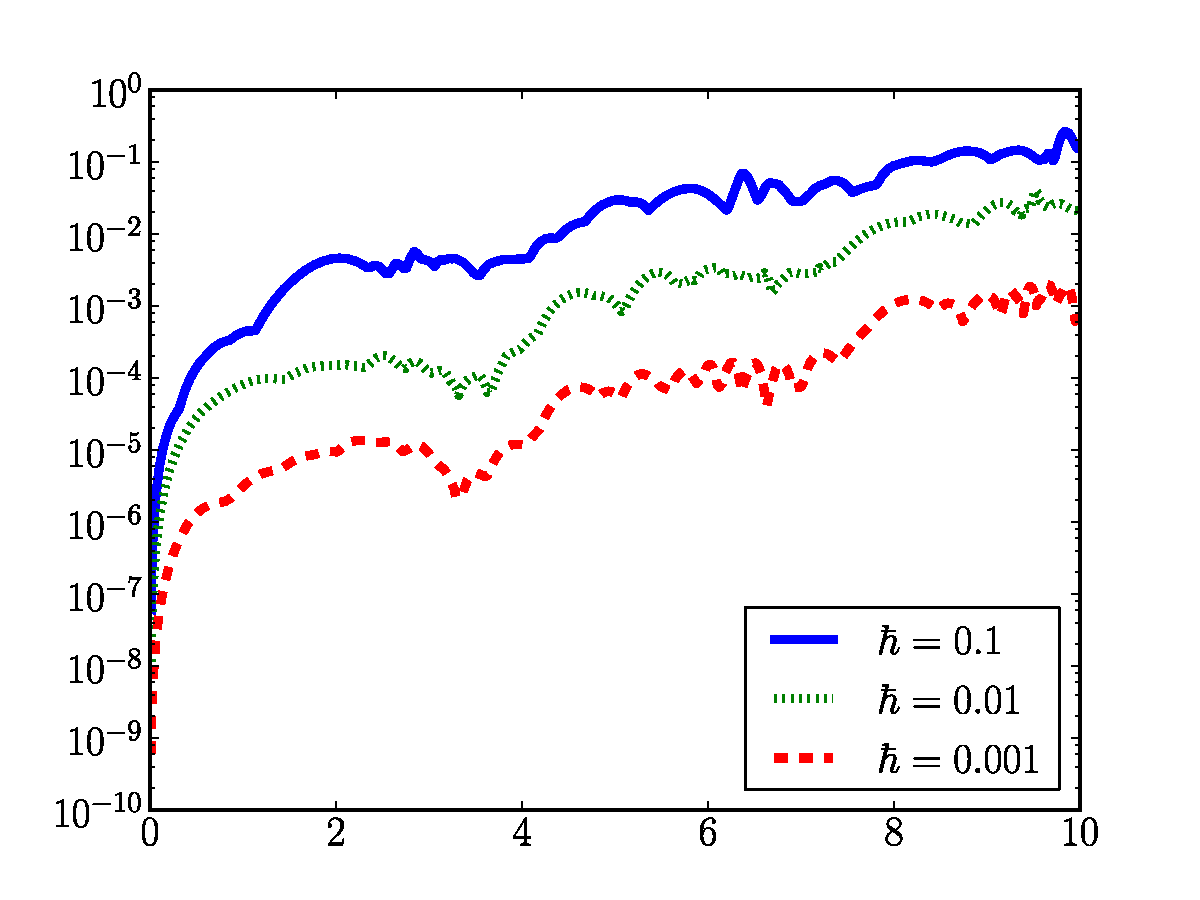
\includegraphics[width=0.5\textwidth]{compH3F12mixA1.pdf}
      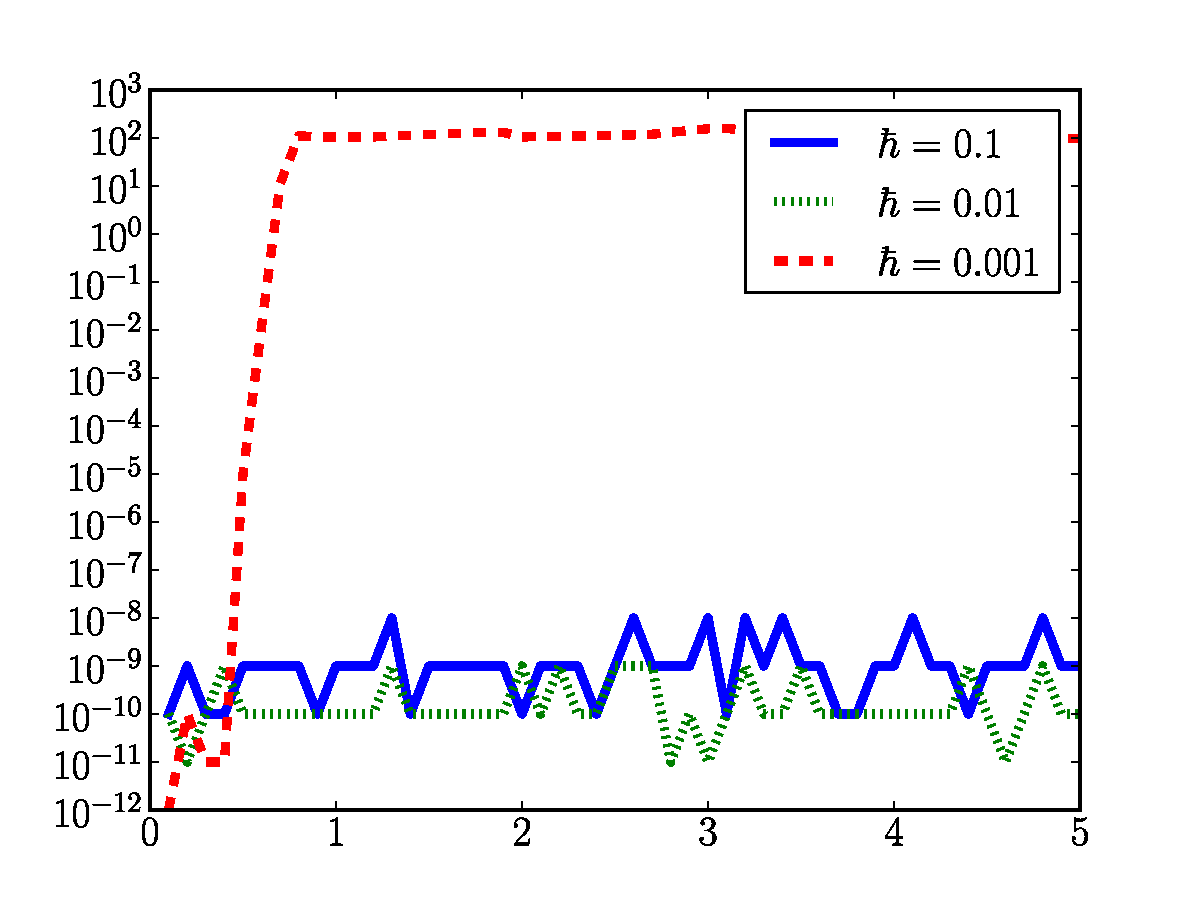
\includegraphics[width=0.5\textwidth]{compFmix1011.pdf}
    }
    % { Error evolution for torsional potential ($d=2$): $20$ wavepackets (left) and
    % $2^{20}$ Fourier functions (right).% for $V(x) = \sum_{j=1}^{d} 1-\cos(x_{j})$.
    % }
    { Evolution of the maximum error in the absolute values of the
      wave function for a torsional potential $V(x) = \sum_{j=1}^{d} 1-\cos(x_{j})$
      with $d=2$:
      semiclassical with $20$ basis functions (left)
      and Fourier with $(2^{r})^{2}$ basis functions for $r=10$ (right).
    }
  }


  \headerbox{References}{name=references,column=0,below=models}{
    \smaller
    \vspace{-1.em}
    \renewcommand\refname{}
    \bibliographystyle{plainnat}
    \bibliography{others,../../references/own}
  }


  \headerbox{Source Code}{name=SourceCode,column=0,below=references,above=bottom}{
    \smaller
    \vspace{-1.em}
    \noindent
    \begin{minipage}{\linewidth}
      \begin{minipage}[c]{0.80\linewidth}
        Python code for semiclassical wavepackets:\\
        \url{https://github.com/raoulbq/WaveBlocksND}
      \end{minipage}\hfill
      \begin{minipage}[c]{0.20\linewidth}
        \hfill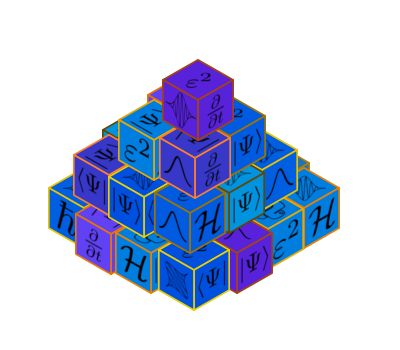
\includegraphics[width=\linewidth]{waveblocks}
      \end{minipage}
    \end{minipage}
  }


  \headerbox{Semiclassical Wavepackets}{name=density,span=2,column=1,row=0}{
    % The semiclassical wavepackets appeared in literature under various names.
    \begin{minipage}[c]{0.6\linewidth}
      We start from a Gaussian wavepacket:
      \begin{shrinkeq}{-1ex}
        \begin{equation*}
          \begin{split}
            \phi_{\vec{0}}^\hbar & [\vec{q},\vec{p},\mat{Q},\mat{P}](\vec{x})\ =
            (\pi\hbar)^{-\frac{d}{4}} (\det \mat{Q})^{-\frac{1}{2}} \,\times \\
            & \exp\left(\frac{i}{2\hbar} \left(\vec{x}-\vec{q}\right)\T \mat{P}\mat{Q}\inv \left(\vec{x}-\vec{q}\right) +
              \frac{i}{\hbar} \vec{p}\T \left(\vec{x}-\vec{q}\right) \right)
          \end{split}
        \end{equation*}
      \end{shrinkeq}
      where $\vec{q}\in \mathbb{R}^d$ and $\vec{p}\in \mathbb{R}^d$ represent the position and momentum,
      respectively, and $\mat{Q}$ and $\mat{P}$ are complex $d\times d$ matrices satisfying some
      compatibility relations.
    \end{minipage}
    \begin{minipage}[c]{0.4\linewidth}
      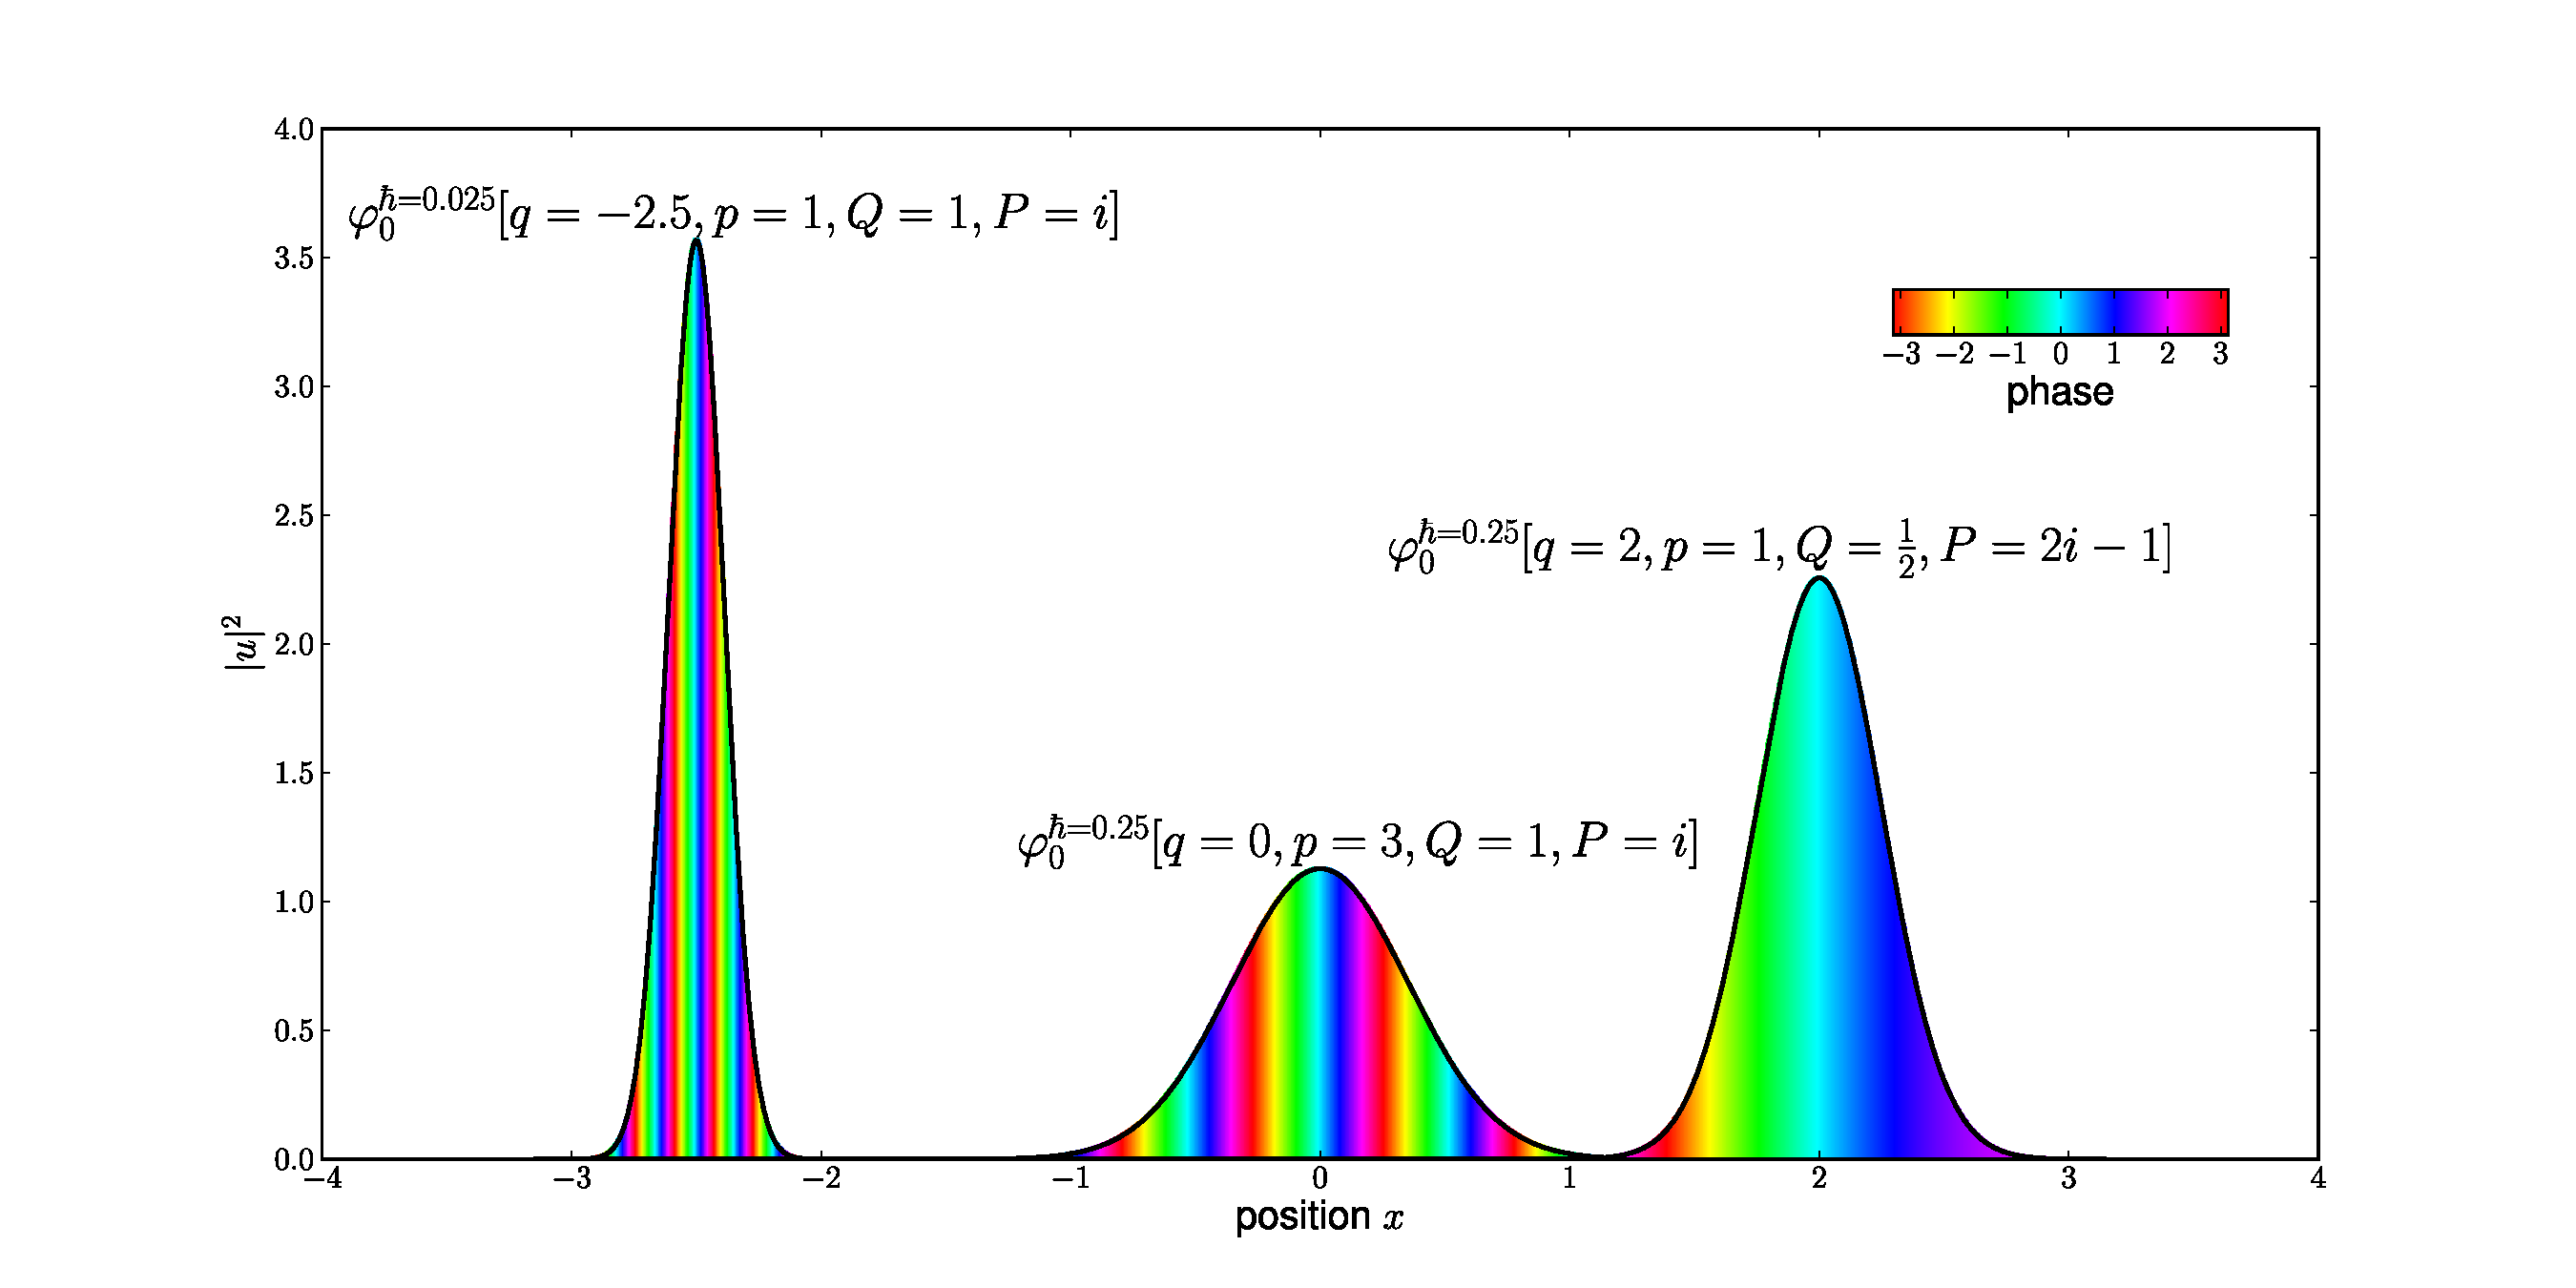
\includegraphics[width=\textwidth]{phip123.pdf}
      % {First member of different families of wavepackets in one dimension.}
    \end{minipage}
    \begin{minipage}[c]{\linewidth}
      Raising and lowering operators $\mathcal{R}$ and $\mathcal{L}$ produce a complete $L^2$-orthonormal
      set of basis functions
      $\phi_{\vec{k}}(\vec{x}) = \phi_{\vec{k}}^\hbar[\vec{q},\vec{p},\mat{Q},\mat{P}](\vec{x})$ (for
      multi-indices $\vec{k} = (k_1,\dots,k_d)$ with non-negative integers $k_j$)
      obeying the three-term recurrence:
      \begin{shrinkeq}{-1ex}
        \begin{equation*}
          \left(\sqrt{k_{j}+1}\phi_{\alert{\vec{k}+\vec{e^j}}}\right)_{j=1}^{d}
          = \sqrt{\frac{2}{\hbar}} \mat{Q}\inv \left(\vec{x}-\vec{q}\right) \phi_{\alert{\vec{k}}} -
          \mat{Q}\inv \conj{\mat{Q}} \left(\sqrt{k_{j}} \phi_{\alert{\vec{k}-\vec{e^j}}}\right)_{j=1}^{d}
        \end{equation*}
      \end{shrinkeq}
    \end{minipage}
    \begin{minipage}[c]{0.5\linewidth}
      \begin{minipage}[c]{\linewidth}
        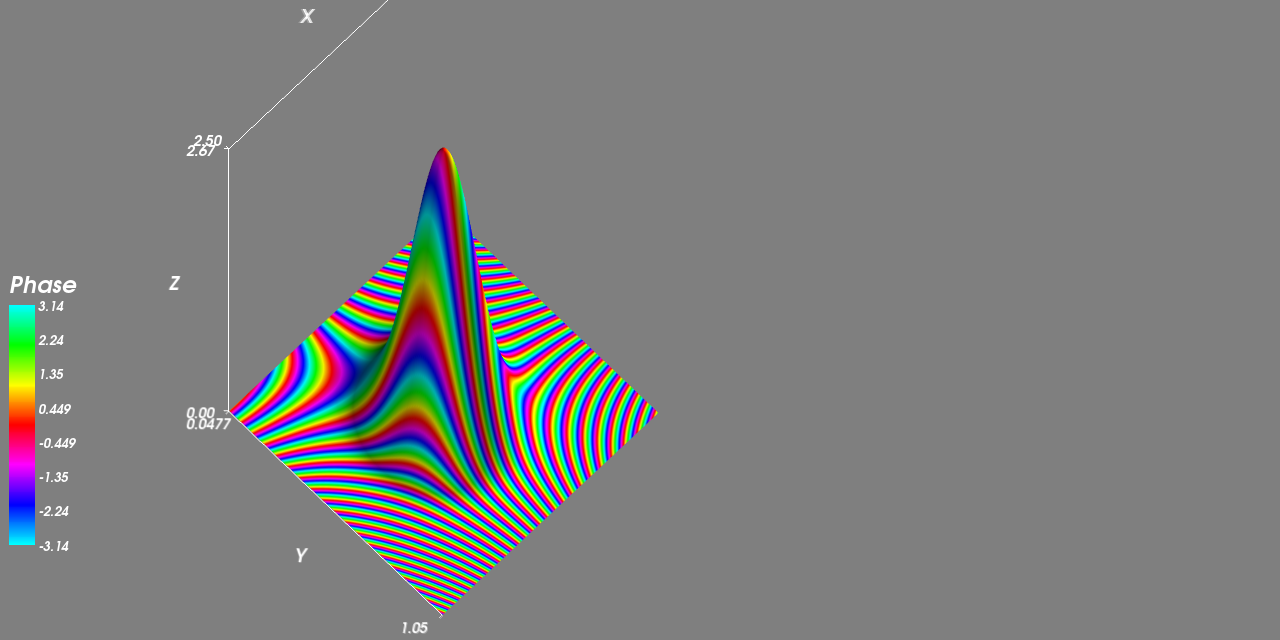
\includegraphics[width=\textwidth]{plot1}
      \end{minipage}
      \hspace*{-0.45\textwidth}
      \begin{minipage}[c]{0.40\textwidth}
        \vspace{1mm}
        { \smaller\white {\smaller
            \begin{align*}
              \vec{k} & = (0,0) \\[-2.5pt]
              \vec{q} & = \left(2, \sqrt{3\varepsilon}\right) \\[-2.5pt]
              \vec{p} & = \left(-\frac{2}{5}, \sqrt{\frac{4\varepsilon}{12}}\right) \\[-2.5pt]
              \mat{Q} & =
              \begin{pmatrix}
                1 & 0\\
                0 & \frac{1}{\sqrt{\frac{4}{5}}}
              \end{pmatrix} \\[-2.5pt]
              \mat{P} & =
              \begin{pmatrix}\smaller
                -2 + i        & -3 \\
                -3 \sqrt{\frac{4}{5}} & i \sqrt{\frac{4}{5}}
              \end{pmatrix} \\[-2.5pt]
              \hbar & = \varepsilon^{2} = \frac{1}{10}
            \end{align*}
          } }
      \end{minipage}
    \end{minipage}
    \begin{minipage}[c]{0.5\linewidth}
      \begin{minipage}[c]{\linewidth}
        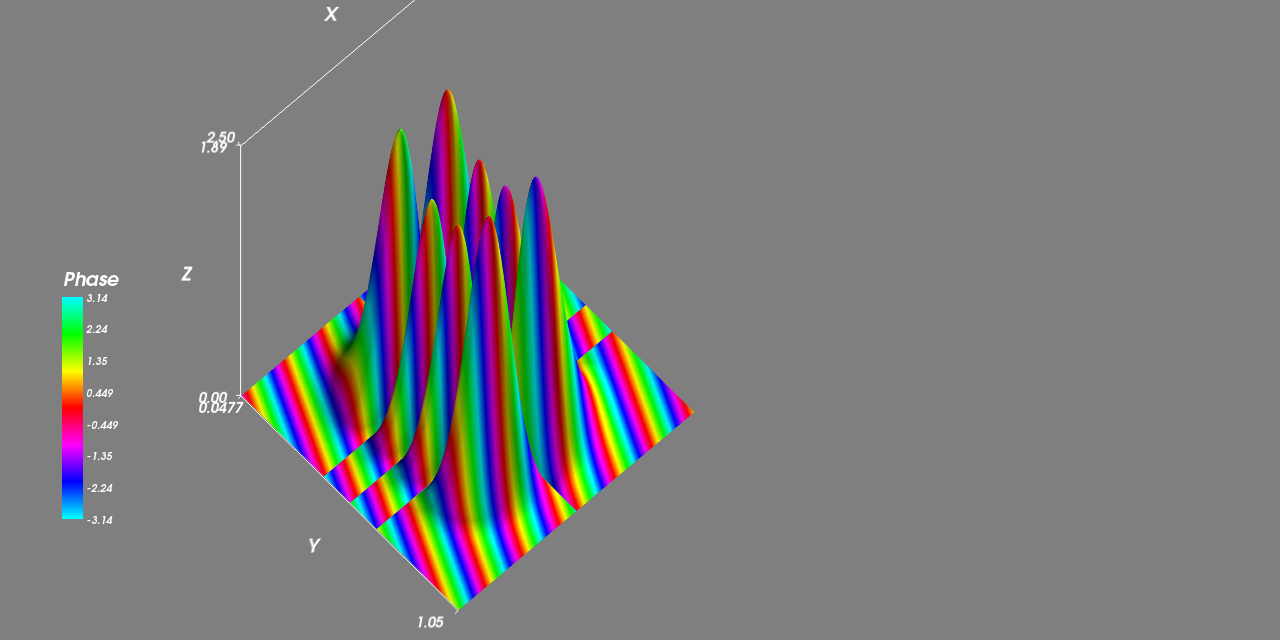
\includegraphics[width=\textwidth]{plot2}
      \end{minipage}
      \hspace*{-0.4\textwidth}
      \begin{minipage}[c]{0.36\textwidth}
        { \smaller\white {\smaller
            \begin{align*}
              \vec{k} & = (1,3) \\
              \vec{q} & = \left(2, \sqrt{3\varepsilon}\right) \\
              \vec{p} & = \left(-\frac{2}{5}, \sqrt{\frac{4\varepsilon}{12}}\right) \\
              \mat{Q} & = \id \\
              \mat{P} & = i\id \\
              \hbar & = \varepsilon^{2} = \frac{1}{10}
            \end{align*}
          } }
      \end{minipage}
    \end{minipage}
    \vspace{-1mm}
  }


  \headerbox{Challenging applications}
  {name=degreeDistribution,span=2,column=1,below=density,above=bottom}{
    When the solution does not remain localized,
    spawning techniques help as demonstrated by \citet{GHJ10b,GHJ10a}
    for a typical tunneling problem and \citet{BGH_natac} in the case of
    nonadiabatic dynamics. The initial value was in all cases a $\phi_{2}$
    on the upper surface.
    % The method based on
    % semiclassical wave packets behave better for smaller $\hbar$ that the
    % standard Fourier method
    % but need many
    % basis-functions for a spreading wave function as in the tunneling problem.
    % \cite{GHJ10a} give a rigorously justified spawning
    % algorithm which specifies
    % when and how to add a new family of semiclassical wave packets during
    % the tunneling in one dimension.
    % \begin{figure}
    %   \centering
    %   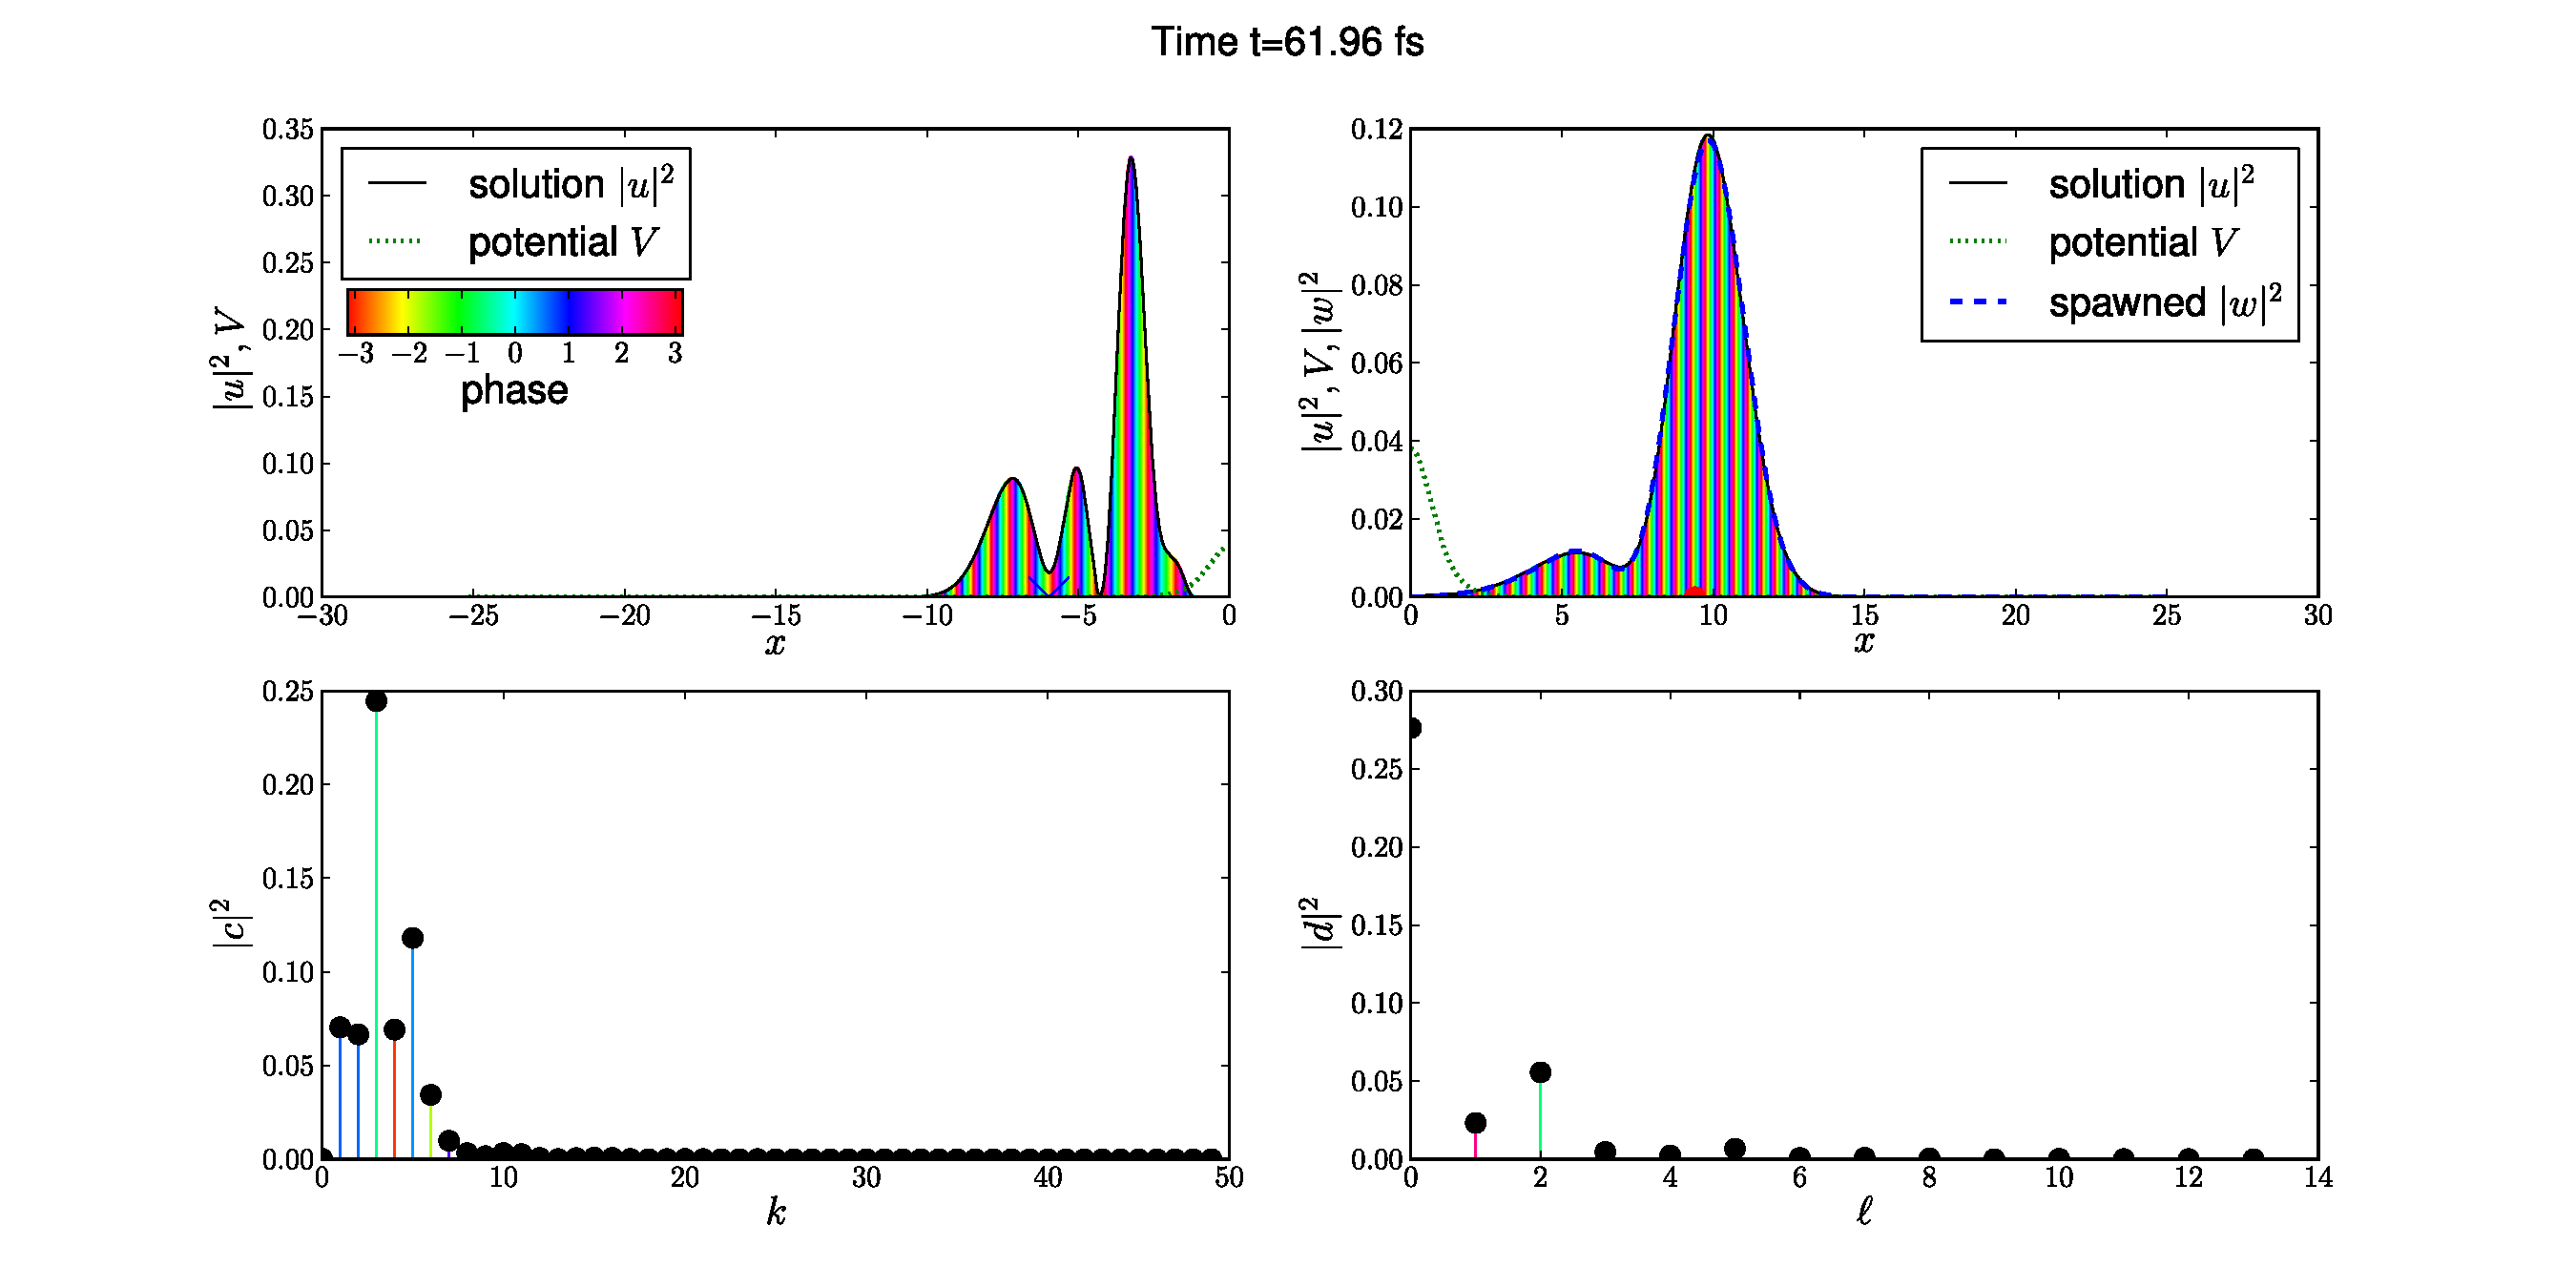
\includegraphics[width=\textwidth,height=12em]{packetFAM00012000.pdf}
    %   {The numerical solution of a standard \alert{tunneling} problem
    %   via wavepackets and with the spawning of a new family (with 13 members)}
    \begin{minipage}[c]{.49\linewidth}
      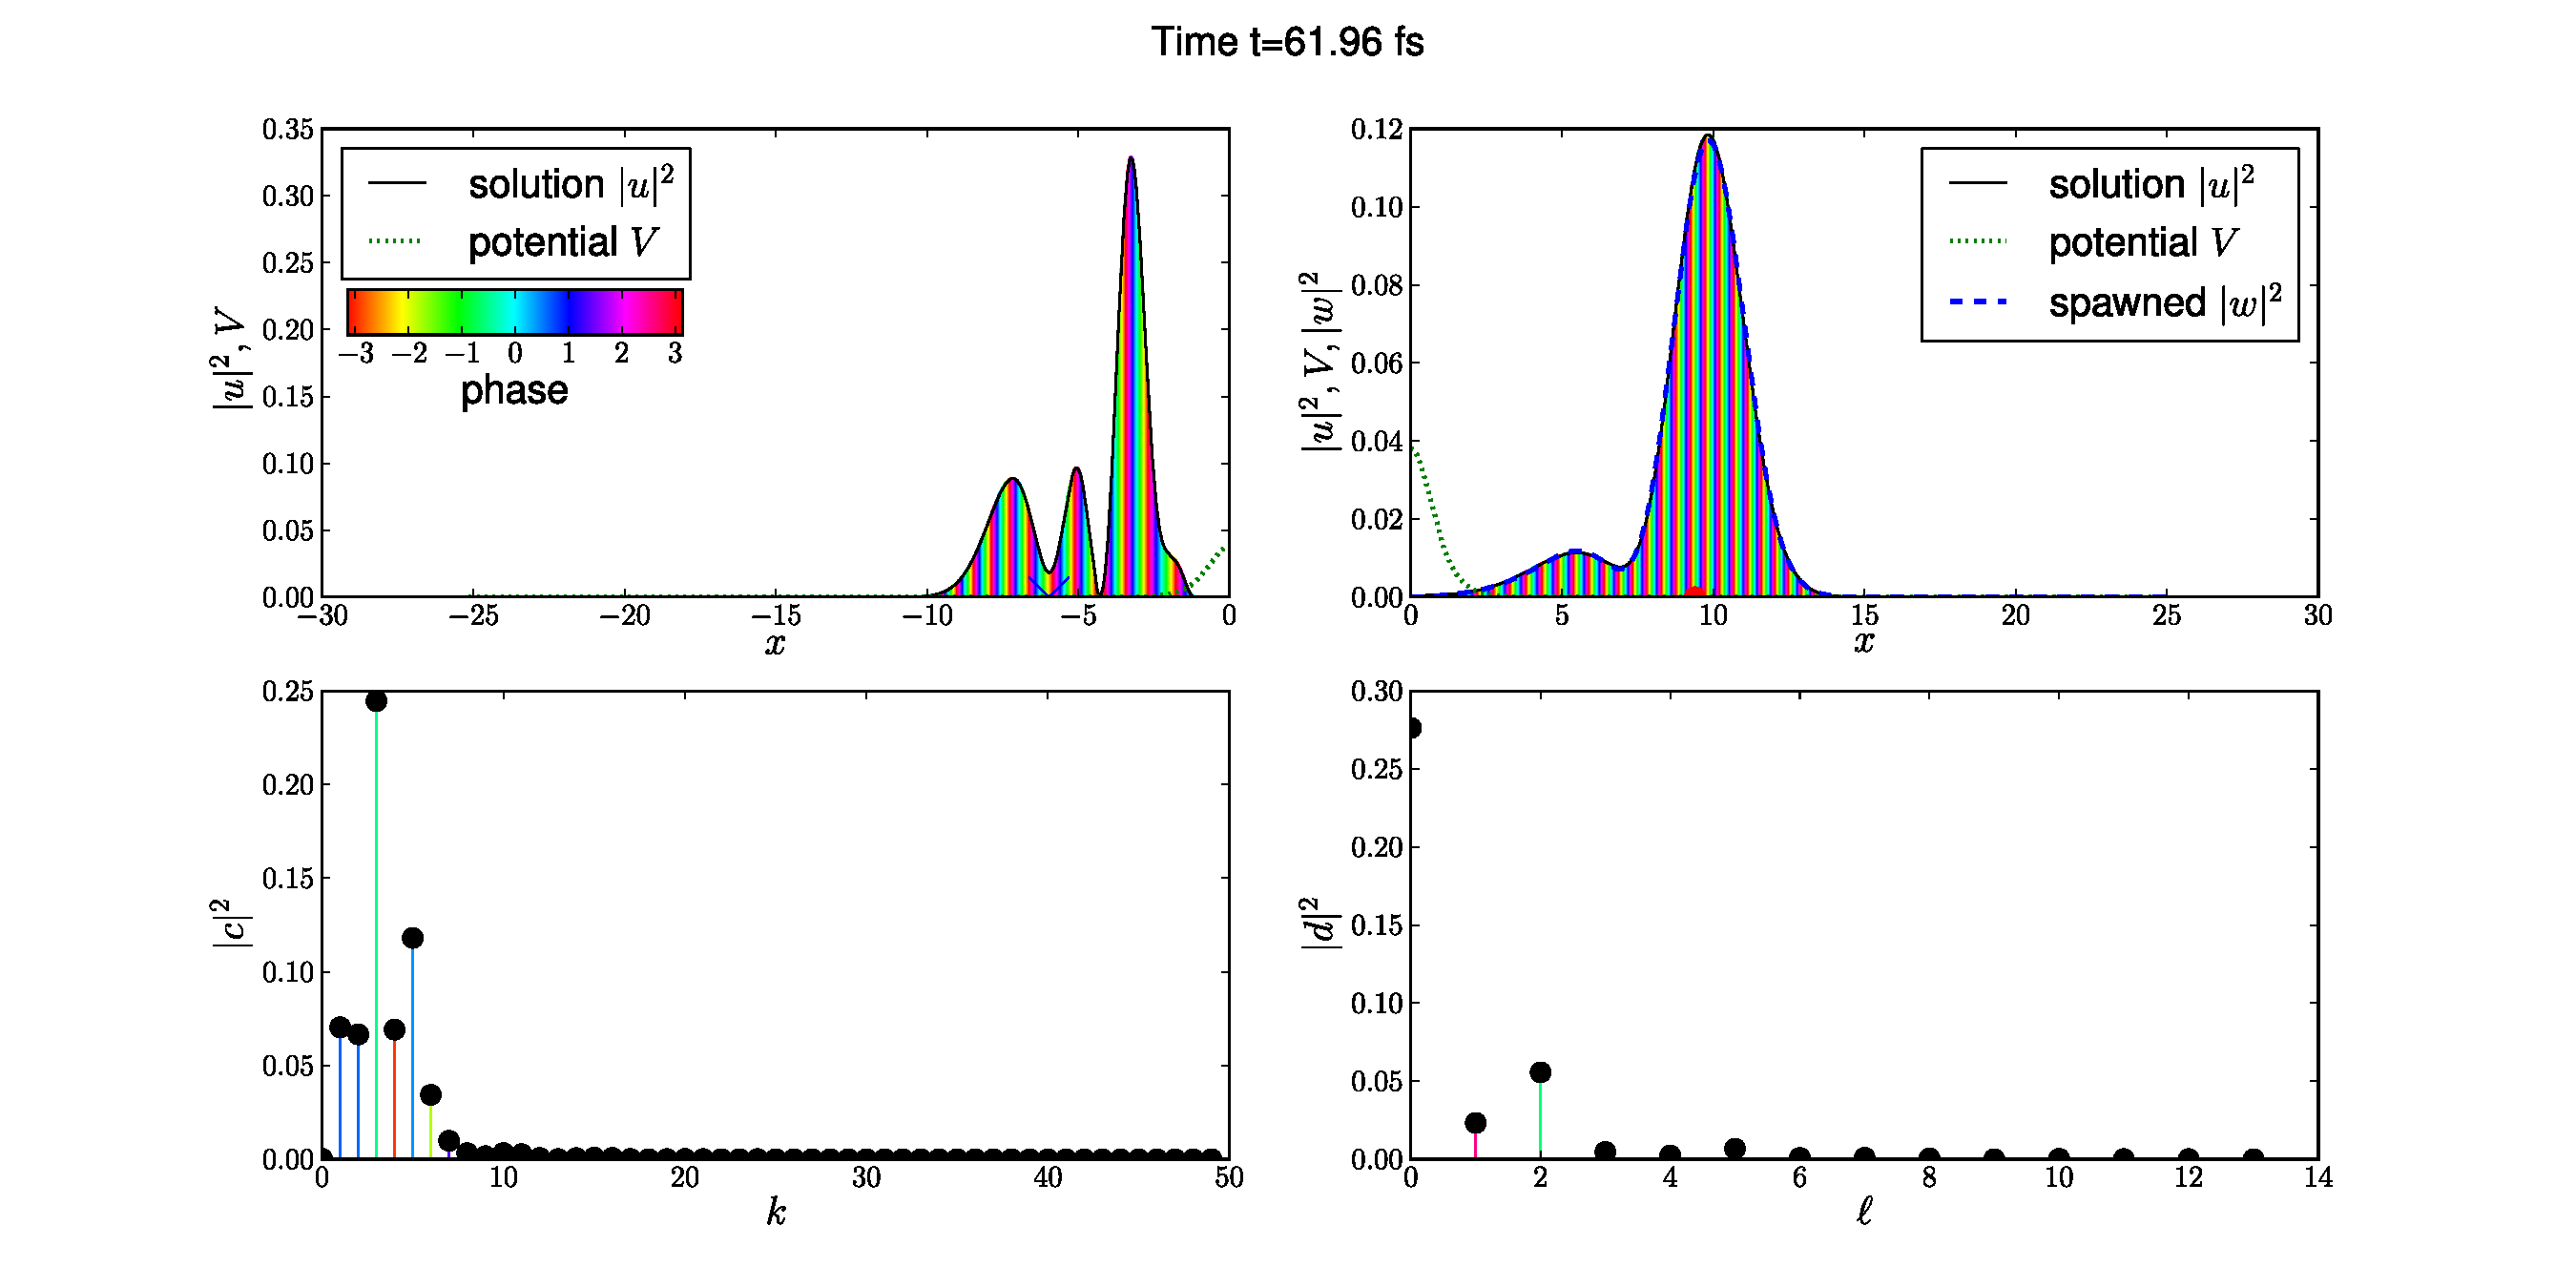
\includegraphics[width=\textwidth]{packetFAM00012000.pdf}
    \end{minipage}
    \begin{minipage}[c]{.5\linewidth}
      Left:
      {numerical solution of a standard \alert{tunneling} problem
        via wavepackets and with the spawning of a new family (with 13 members)}\\
      Below: results for
      \alert{non-adiabatic} dynamics,      e.g. avoided crossing:
      \begin{eqnarray*}\label{III:tanhex}
        V(x,\delta)& = &
        \begin{pmatrix}
          \frac12\tanh(x) & \frac12\delta \\
          \frac12\delta   & -\frac12\tanh(x)
        \end{pmatrix}
      \end{eqnarray*}
      with eigenvalues $\pm\frac12\sqrt{\delta^{2}+\tanh(x)^{2}}$.
      % \begin{minipage}[c]{0.4\linewidth}
      %   \begin{figure}[htbp]
      %     \centering
      %     \includegraphics[width=\textwidth]{actanhEL.pdf}
      %   \end{figure}
      % \end{minipage}
    \end{minipage}
    \centerline{
      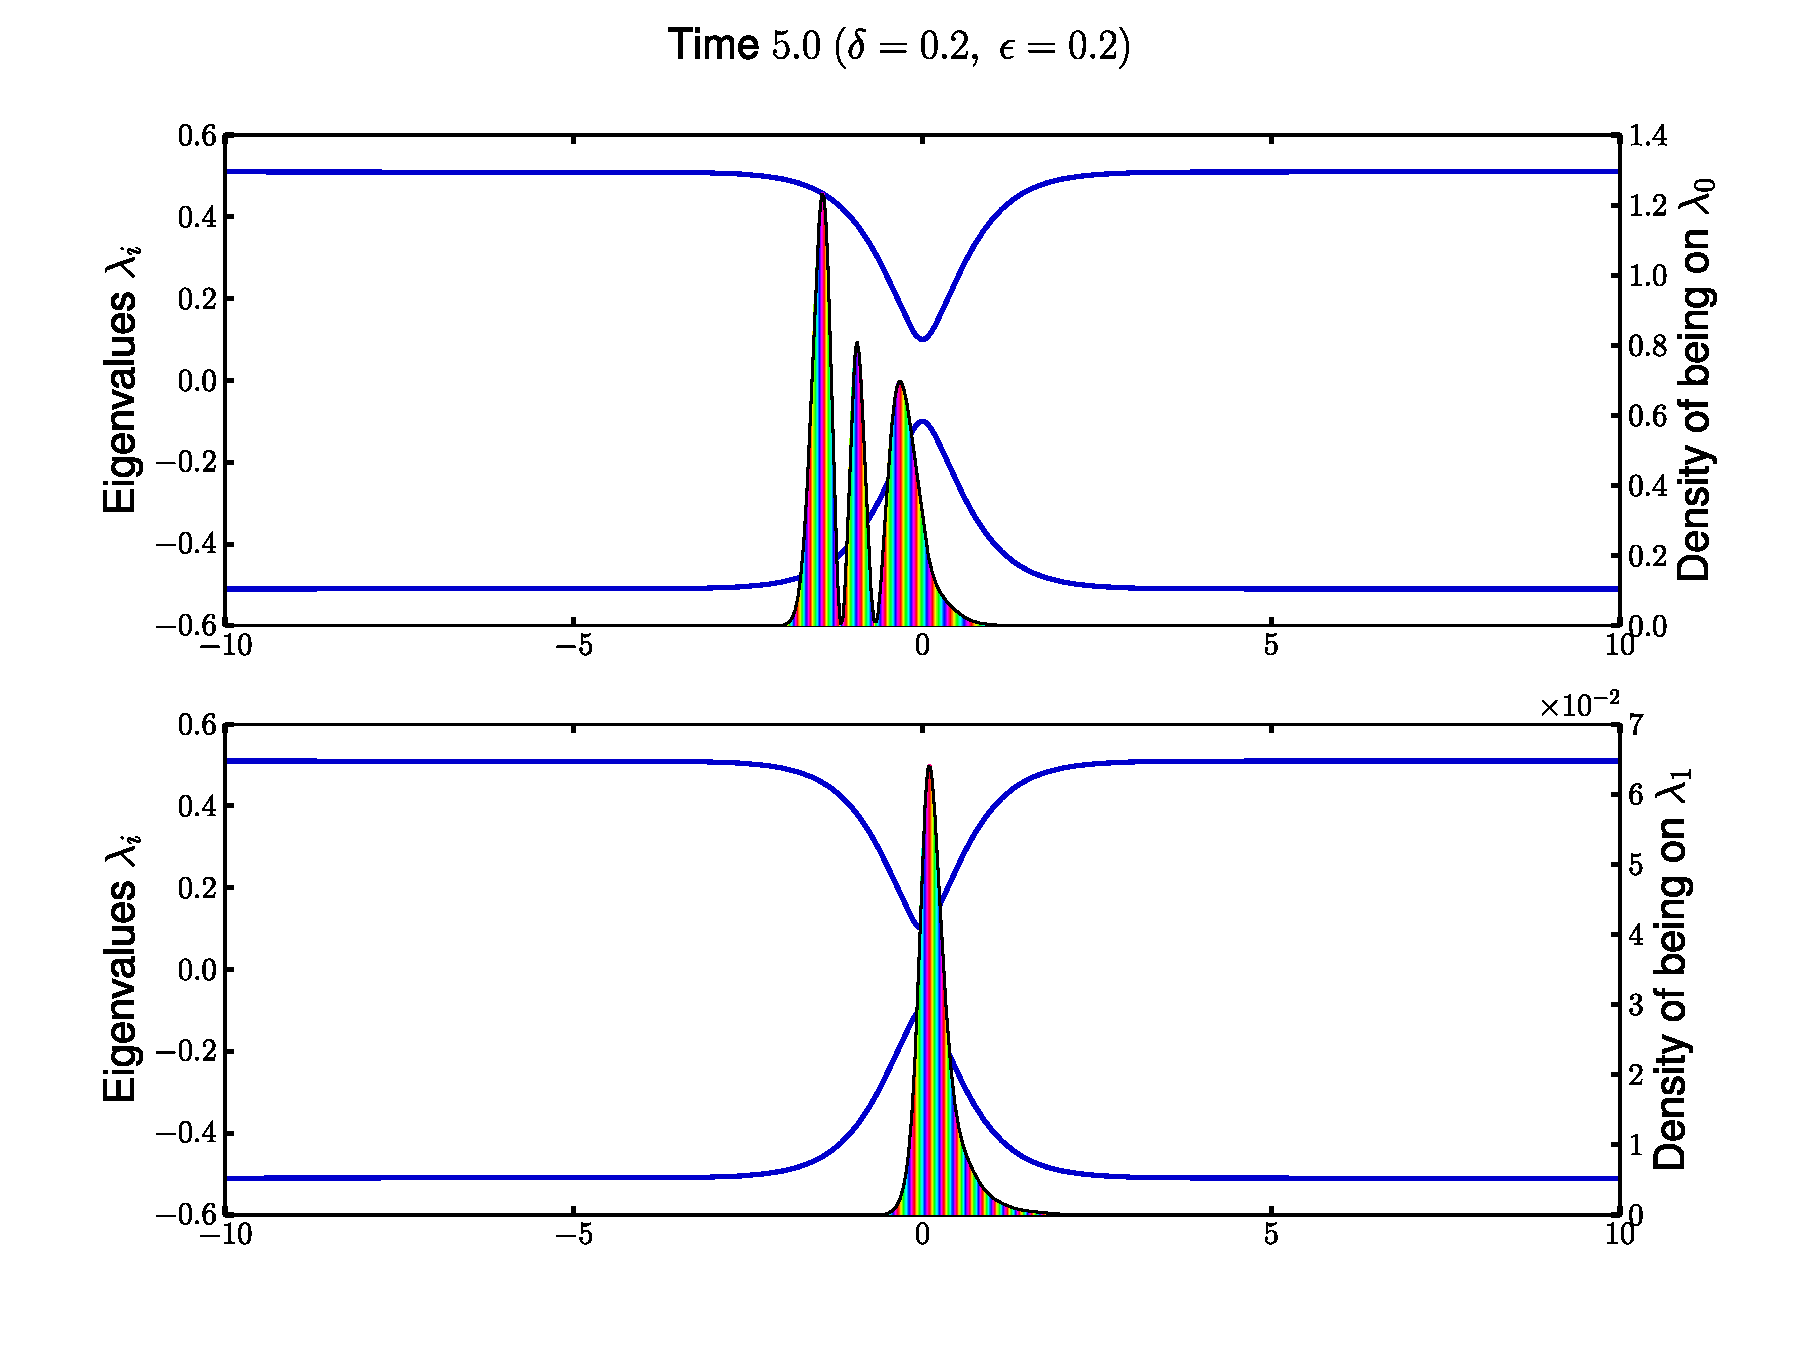
\includegraphics[width=0.35\textwidth,height=13em]{ParametersHeps0_2d1_0eS2PotAndWwave00250.pdf}
      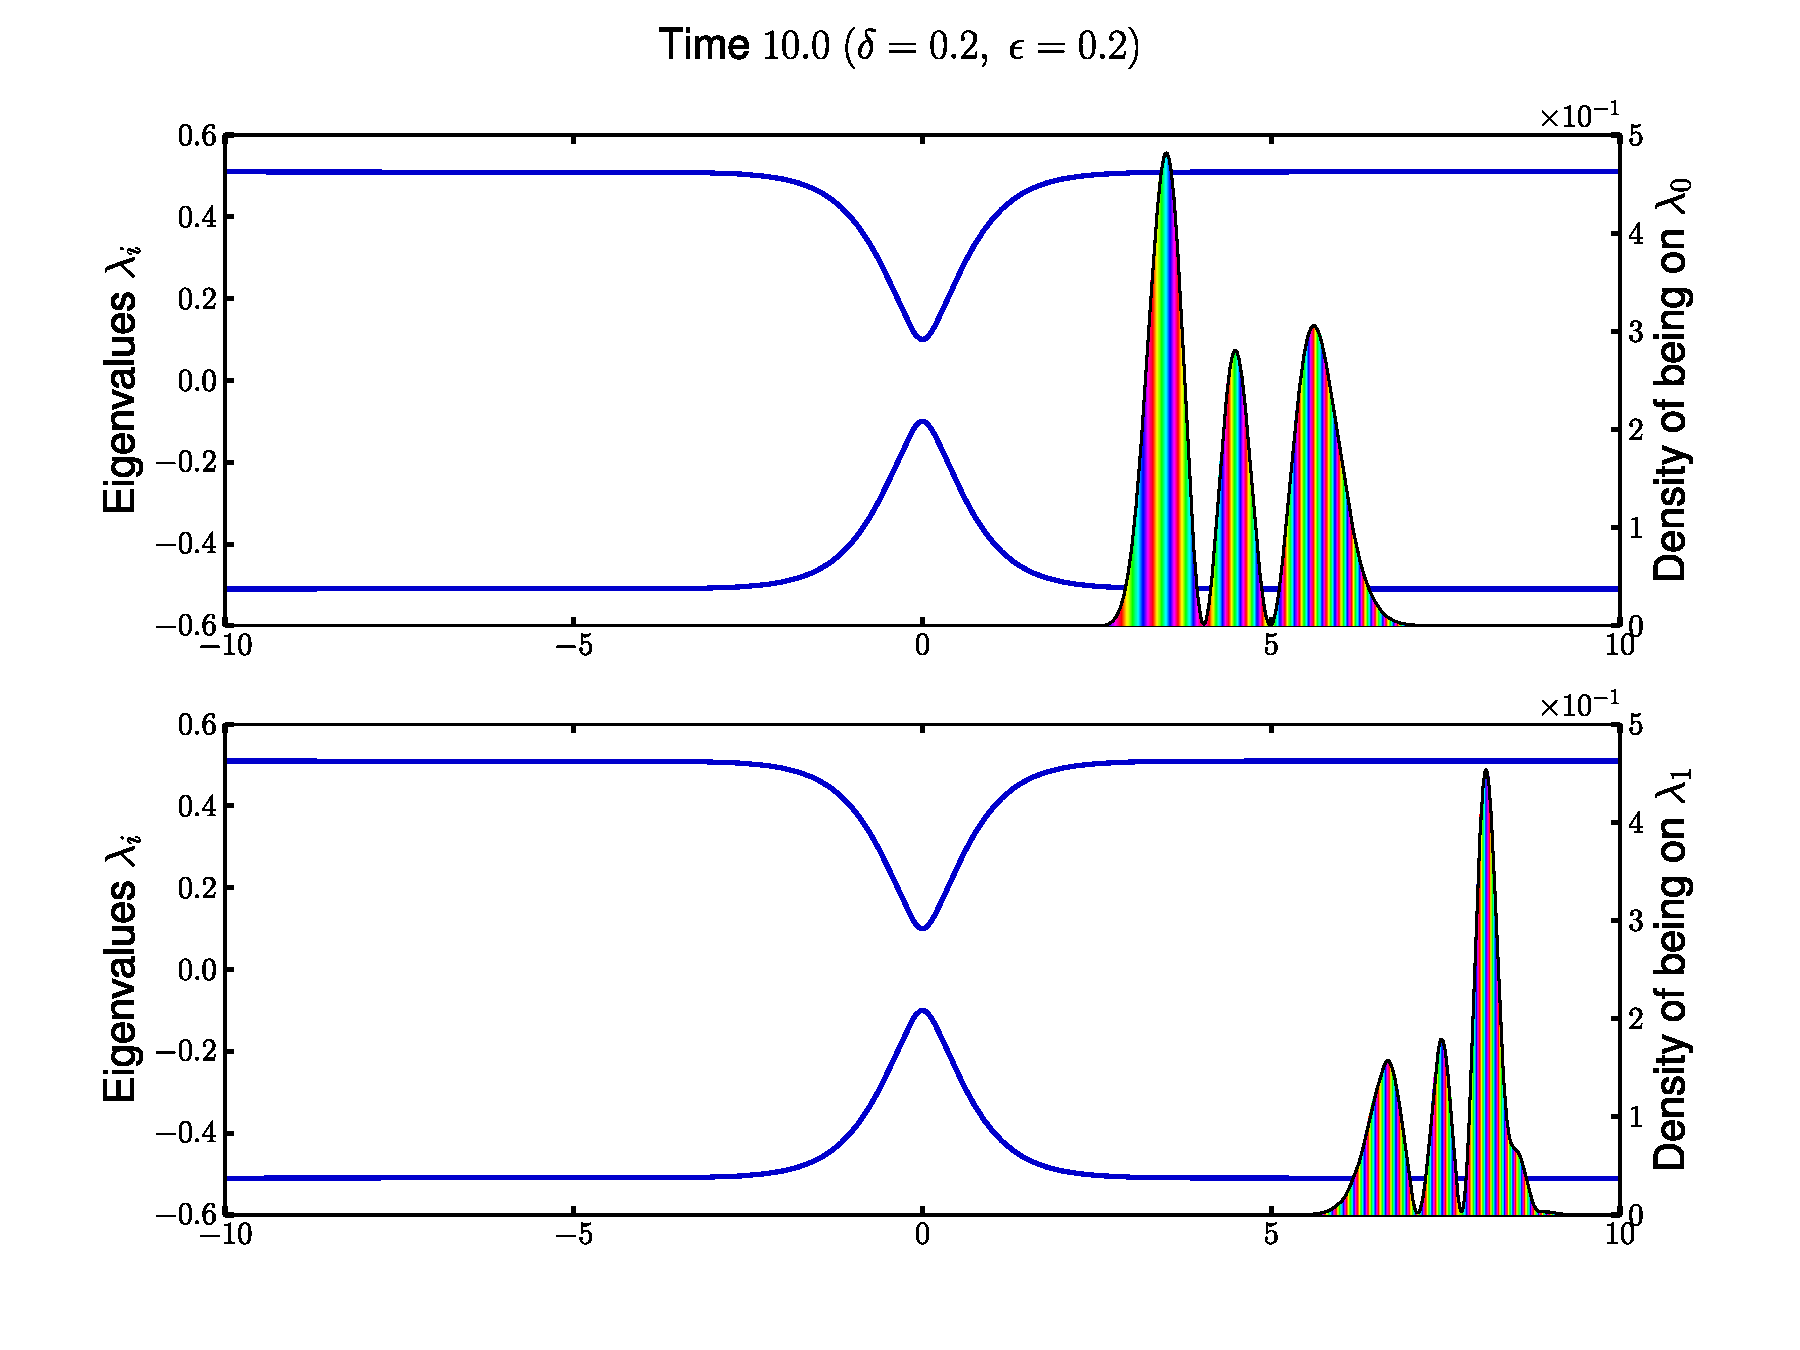
\includegraphics[width=0.35\textwidth,height=13em]{ParametersHeps0_2d1_0eS2PotAndWwave00500.pdf}
      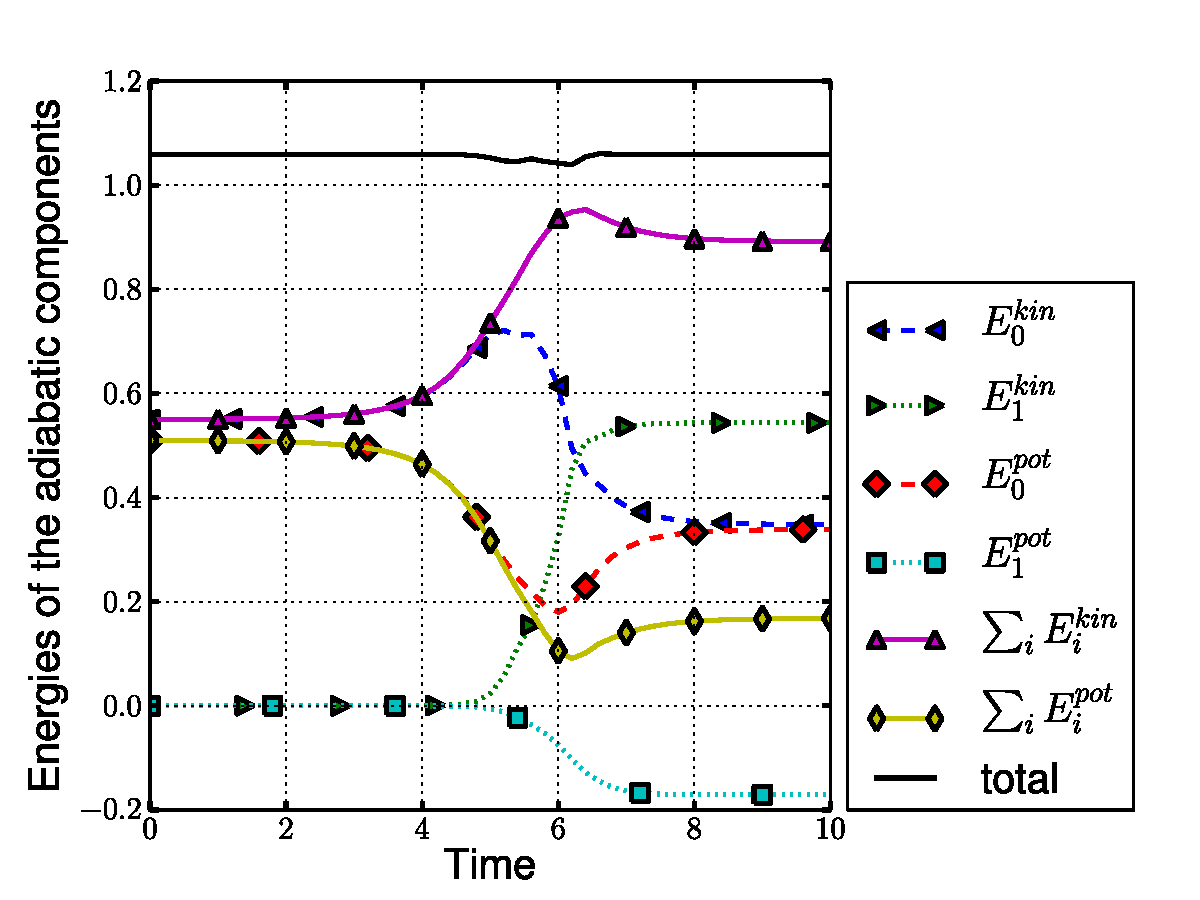
\includegraphics[width=0.3\textwidth,height=13em]{ParametersHeps0_2d1_0eS2energies.pdf}
    }
    { Position space plot of the probability density of being on the upper energy level
      $\lambda_{0} = E_{\cal A}(\cdot,\delta)$ and on the lower energy level
      $\lambda_{1} = E_{\cal B}(\cdot,\delta)$ in the case of a small energy gap
      $\delta=\varepsilon=0.2$ (i.e. $\hbar = 0.04$). The left scale refers to the energy
      levels, while the right scale refers to the squared absolute values of the components
      $\Phi_{\cal A}$ (upper) and $\Phi_{\cal B}$ (lower) on the two levels.}
    \centerline{
      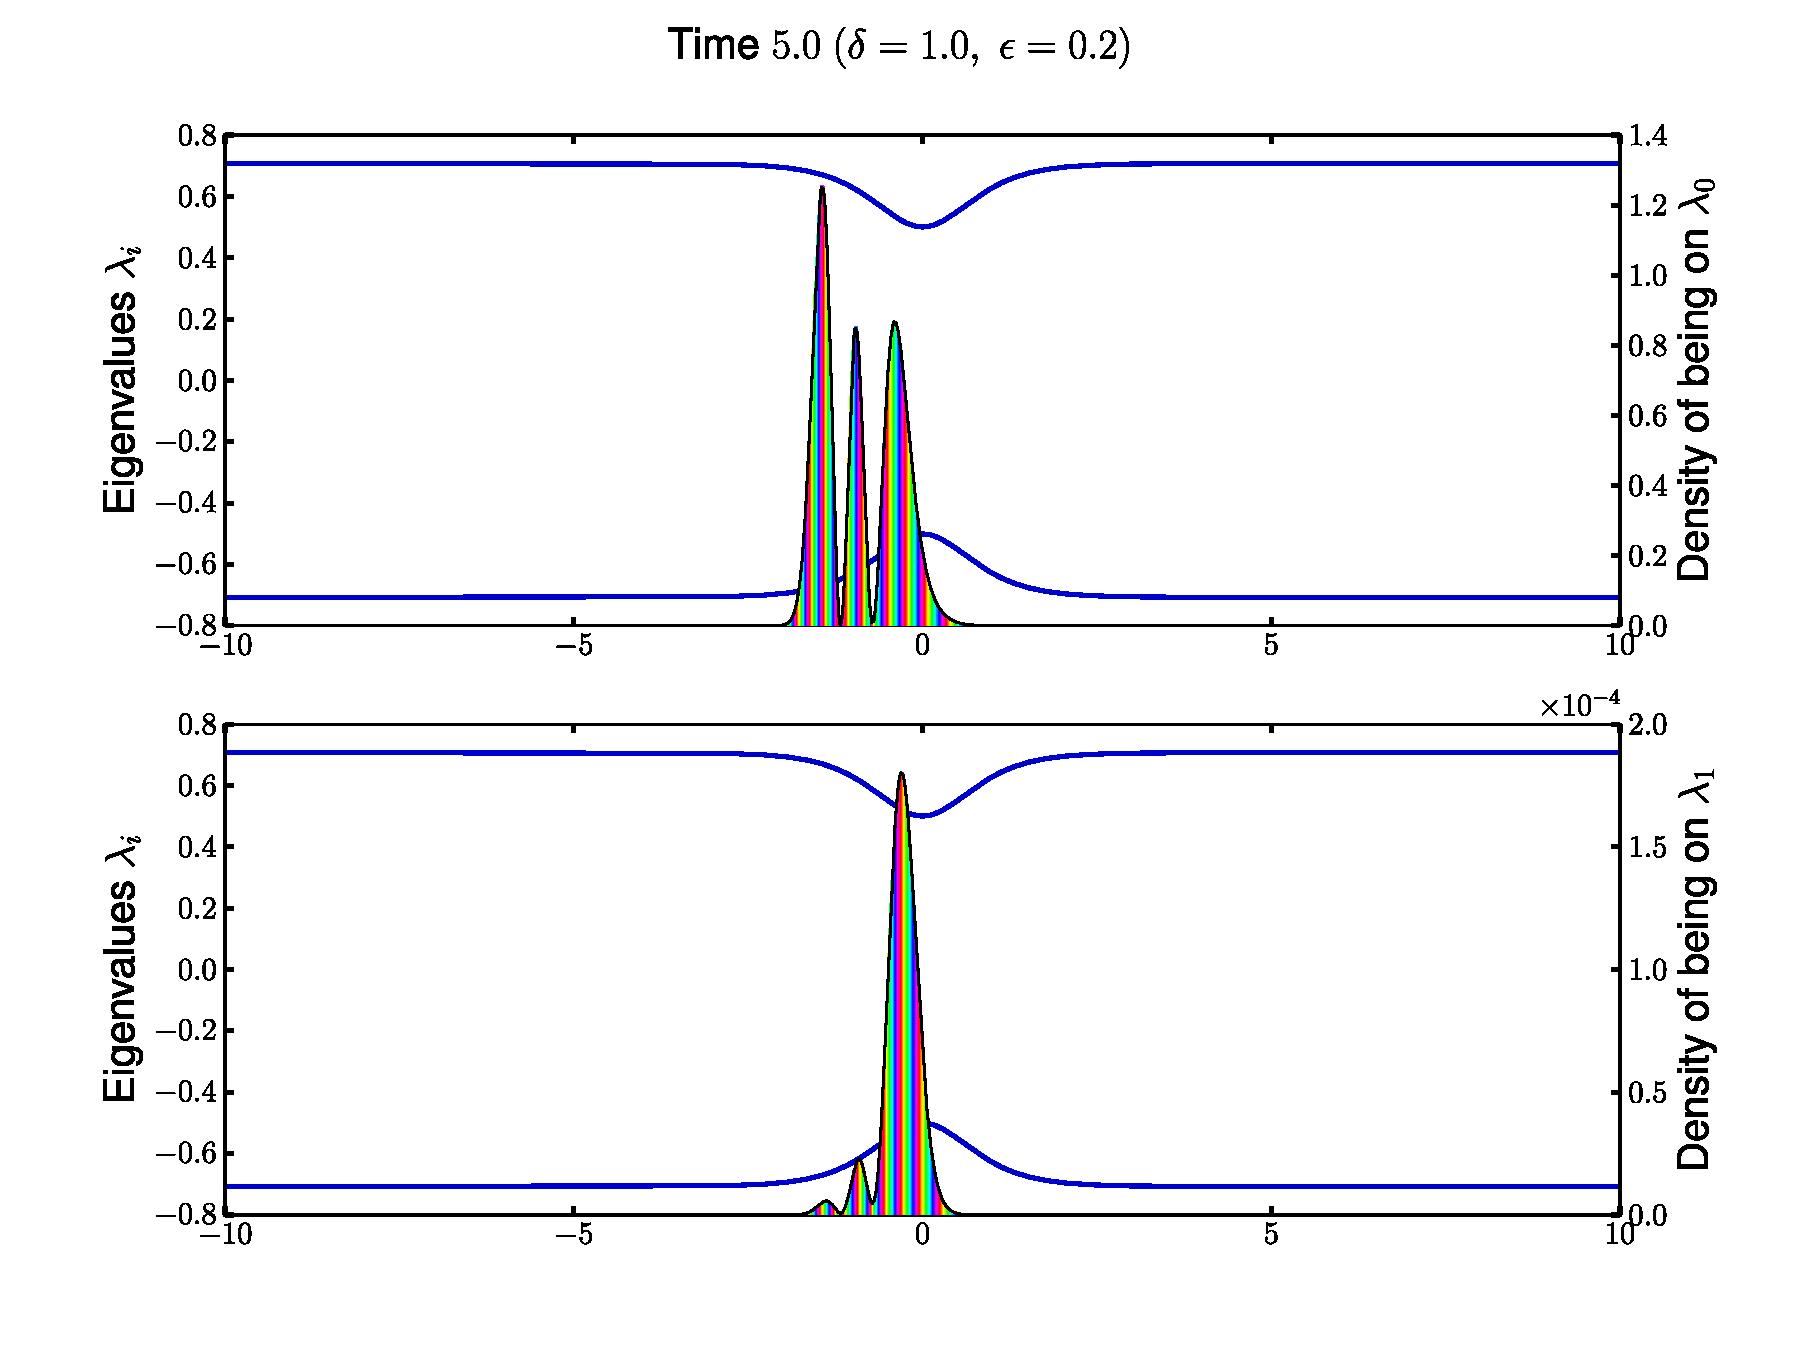
\includegraphics[width=0.35\textwidth,height=13em]{ParametersHeps0_2d5_0eS2PotAndWwave00250.pdf}
      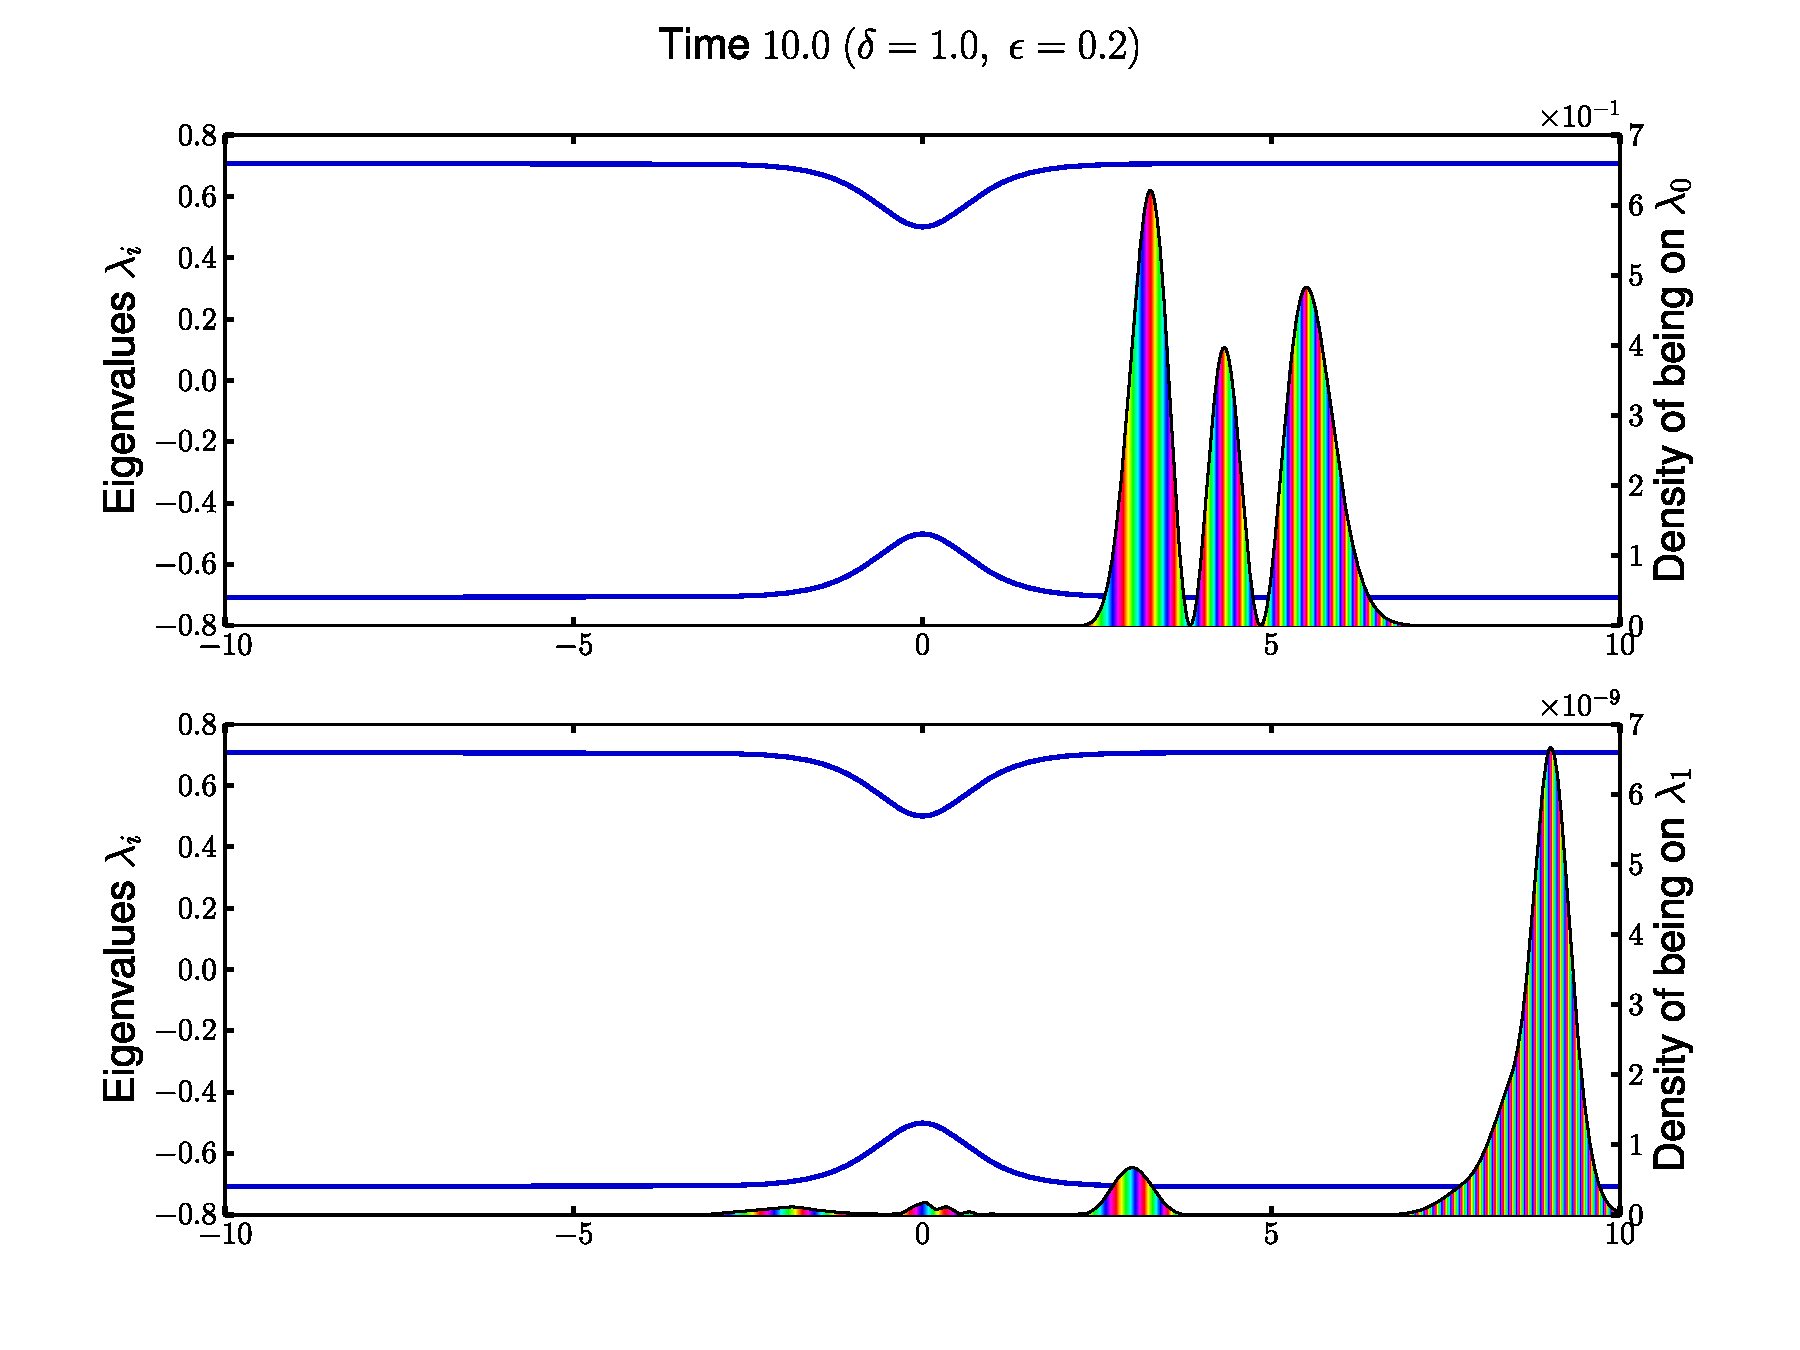
\includegraphics[width=0.35\textwidth,height=13em]{ParametersHeps0_2d5_0eS2PotAndWwave00500.pdf}
      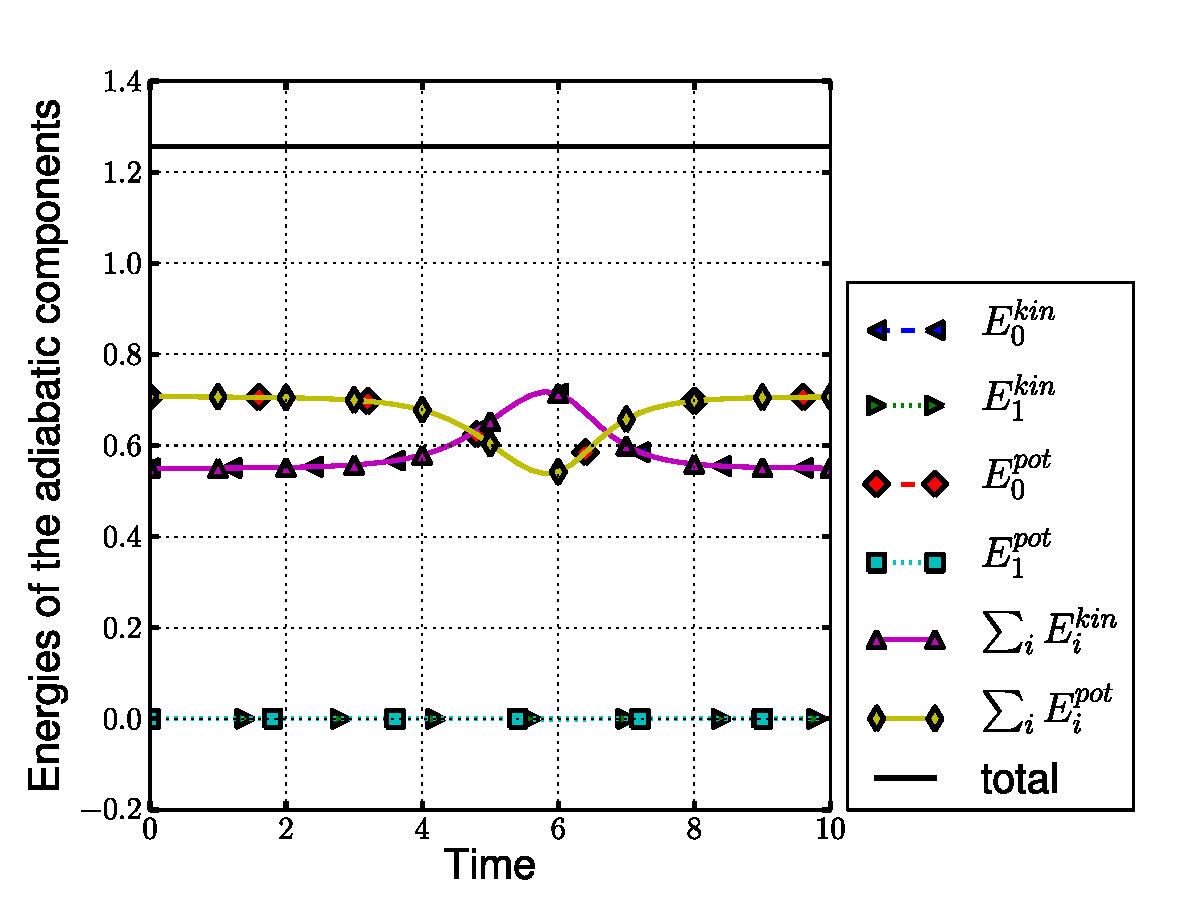
\includegraphics[width=0.3\textwidth,height=13em]{ParametersHeps0_2d5_0eS2energies.pdf}
    }
    { Position space plot  of the probability density of being on the upper energy level
      $\lambda_{0} = E_{\cal A}(\cdot,\delta)$ and on the lower energy level
      $\lambda_{1} = E_{\cal B}(\cdot,\delta)$ in the case of a large energy gap
      $\delta=5\varepsilon=1$. The left scale refers to the energy levels, while the right
      scale refers to the squared absolute values of the components $\Phi_{\cal A}$ (upper)
      and $\Phi_{\cal B}$ (lower) on the two levels. Note the different magnitudes!}
  }

\end{poster}
\end{document}
